\documentclass[a4paper]{article}

\usepackage[english]{babel}
\usepackage[utf8]{inputenc}
\usepackage{amsmath}
\usepackage{graphicx}
\usepackage{epsfig}
\usepackage{amsfonts}
\usepackage[ruled,vlined]{algorithm2e}
\usepackage{bbm}
\usepackage{pythonhighlight}
\usepackage[colorinlistoftodos]{todonotes}
\usepackage[hidelinks]{hyperref}
\usepackage[margin=1.3in]{geometry}

\DeclareMathOperator*{\argmax}{arg\,max}
\DeclareMathOperator*{\argmin}{arg\,min}

\title{Deep Learning Reviews}

\author{Ao Zhang}

%\date{June 2015}

\newcommand{\gfigure}[4]
{
	\begin{figure}
      \begin{center}
          \includegraphics[#3]{#4}
          \caption{#1}
          \label{Figure:#2}
      \end{center}
    \end{figure}
}
\newcommand{\figref}[1]{Figure~\ref{Figure:#1}}

\begin{document}
\maketitle


\section{Some Definitions}

\begin{itemize}
	\item \textbf{Supervised Learning}: Given $\mathcal{D} = \{ (x_i, y_i): i = 1, 2, ..., n \}$, develop a program that predicts $Y$ from $X$, or finds how $Y$ depends on $X$.
	\item \textbf{Unsupervised Learning}: Given $\mathcal{D} = \{ x_i: i = 1, 2, ..., n \}$, develop a program that finds the structure in $X$, or generates an (new) $X$ that conforms to the structure.
	\item \textbf{Reinforcement Learning}: Suppose there is an ``environment'' which can interact with an agent by changing the ``state'' and generating a reward for the agent. Develop an agent program that maximize some accumulated reward it receives.
	\item \textbf{Model}: A restricted family $\mathcal{H}$ of hypotheses. 
	\begin{equation}
		Y = f(X; \hat{\theta})
	\end{equation}
	\item \textbf{Parametric Models}: Models have a fixed number of parameters, independent of sample size.
	\item \textbf{Non-Parametric Models}: The number of parameters increases with sample size. (usually not considered.)
	\item \textbf{Loss Functions}: A model is usually characterized by Loss Function $\mathcal{L}(\theta)$ over the space $\Theta$ of model parameters $\theta$. An example using Mean Square Error (MSE) is shown as below.
	\begin{equation}
		\hat{\theta} := \argmin_{\theta \in \Theta} \mathcal{L}(\theta) = || Y - X \theta ||^2 \label{lf}
	\end{equation}
	\item \textbf{Gradient Descent (GD)}: Based on Equation~\ref{lf},
	\begin{align}
		{\theta}^{new} &= {\theta}^{old} - \lambda \frac{d \mathcal{L}}{d \theta} ({\theta}^{old}) \\
		&= {\theta}^{old} + \lambda \frac{1}{N} \sum_{i=1}^{N} 2 (y_i - {\theta}^{old} x_i) x_i
	\end{align}
	\item \textbf{Stochastic Gradient Descent (SGD)}: Based on Equation~\ref{lf},
	\begin{equation}
		{\theta}^{new} = {\theta}^{old} + \lambda 2 (y_i - {\theta}^{old} x_i) x_i
	\end{equation}
	\item \textbf{Mini-Batched SGD}: Based on Equation~\ref{lf},
	\begin{equation}
		{\theta}^{new} = {\theta}^{old} + \lambda \frac{1}{|\mathcal{B}|} \sum_{(x, y) \in \mathcal{B}} 2 (y - {\theta}^{old} x) x
	\end{equation}
\end{itemize}

\section{Initalization}

Good intialization of the model parameters will prevent exploding or vanishing gradients. A too-large initialization leads to exploding gradients and a too-small initialization leads to vanishing gradients.

Rules of appropriate intialization:
\begin{itemize}
	\item The mean of the activations should be zero.
	\item The variance of the activations should stay the same across every layer.
\end{itemize}

Typical intialization methods:
\begin{itemize}
	\item Ramdom Norm (Gaussian) Distribution:
	\item \textbf{Xavier Intialization (most popular)}: Use a normal distribution with $\sigma = \sqrt{\frac{2}{n_{in} + n_{out}}}$; Or use a uniform distribution with a range $r = \sqrt{\frac{6}{n_{in} + n_{out}}}$
	\item Bias Initialization: often assign them to $0$.
\end{itemize}

\section{Activation Functions}

\begin{itemize}
	\item \textbf{Sigmoid Function}:
	\begin{align}
		\sigma (x) &= \frac{1}{1 + e^{-x}} \\
		\sigma^{\prime} (x) &= \sigma (x) (1 - \sigma(x))
	\end{align}
	\item \textbf{Softmax Function}: 
	\begin{equation}
		\text{softmax} (x_i) = \frac{e^{x_i}}{\sum_{j=1}^{K} e^{x_j}},\,\,\,\, x_i \in \mathbb{R}^K
	\end{equation}
	\item \textbf{Rectified Linear Unit (ReLU)}:
	\begin{equation}
		\text{ReLU} (x) = \max \{ x, 0 \}
	\end{equation}
	\item \textbf{Leaky ReLU}:
	\begin{equation}
		\text{ReLU} (x) = \max \{ x, 0 \} + \alpha \min \{ x, 0 \},\,\,\,\, \alpha > 0
	\end{equation}
	\item \textbf{Hyperbolic Tangent Function}:
	\begin{equation}
		\text{tanh} (x) = \frac{e^x - e^{-x}}{e^x + e^{-x}}
	\end{equation}
	\item \textbf{Softplus}:
	\begin{equation}
		\text{softplus} (x) = \log (1 + e^x)
	\end{equation}
\end{itemize}

\section{Normalization}  

\textbf{Batch Normalization}: 
\begin{align}
	\text{bn}_{k, j} (a) &= \frac{a - \mathbb{E} (X^{(k)}[j])}{\text{VAR} (X^{(k)}[j])} \\
	\mathbb{E} (X^{(k)}[j]) &\approx \mu_{\mathcal{B}, j}^{(k)} = \frac{1}{|\mathcal{B}|} \sum_{j \in \mathcal{B}} x^{(k)}[j] \\
	\text{VAR} (X^{(k)}[j]) &\approx s_{\mathcal{B}, j}^{(k)} = \frac{1}{|\mathcal{B}|} \sum_{j \in \mathcal{B}} (x^{(k)}[j] - \frac{1}{|\mathcal{B}|})^2
\end{align}
where, $\mathcal{B}$ means batched data; $X^{(k)}$ stands for input data to the $k$-th layer.

Reason why Batch Normalization works: Avoiding Internal Covariate Shift. Imagine the model is described in a Marcov Chain mode,
\begin{equation}
	X^{(0)} \leftarrow X^{(1)} \leftarrow X^{(2)} \leftarrow X^{(3)} \leftarrow ... \leftarrow X^{(n)}
\end{equation}
Therefore, the output probability of the $k$-th layer is a conditional distribution from previous prediction probability. As the input to the $1$-st layer is already a batched data, the conditional distribution learning starts from the beginning. When using SGD to update parameters from $\theta^{old}$ to $\theta^{new}$, the covariance of the $k$-th layer parameters will be shifted. This phenomenon is called ``Internal Covariate Shift''. It can sometimes cause vanishing gradient. Using Batch Normalization can pretty much tackle the problem, as it re-scale the vanishing predictions to $[-1, 1]$.

Another reason why Batch Normalization works: It just be smoothing the loss landscape.
 
\section{Regularization}

First, we need to review what is \textbf{Overfitting} and what is \textbf{Underfitting}. Some definitions need to be introduced at the beginning.
\begin{itemize}
	\item \textbf{In-Sample Error}: Also known as \textbf{training error}, notation $E_{in}$.
	\item \textbf{Out-Sample Error}: Also known as \textbf{testing error}, notation $E_{out}$.
	\item \textbf{Generalization Gap}: Notation $E_{gen}$
	\begin{equation}
		E_{gen} = E_{out} - E_{in}
	\end{equation}
\end{itemize}

\begin{figure}[h]
	\centering
	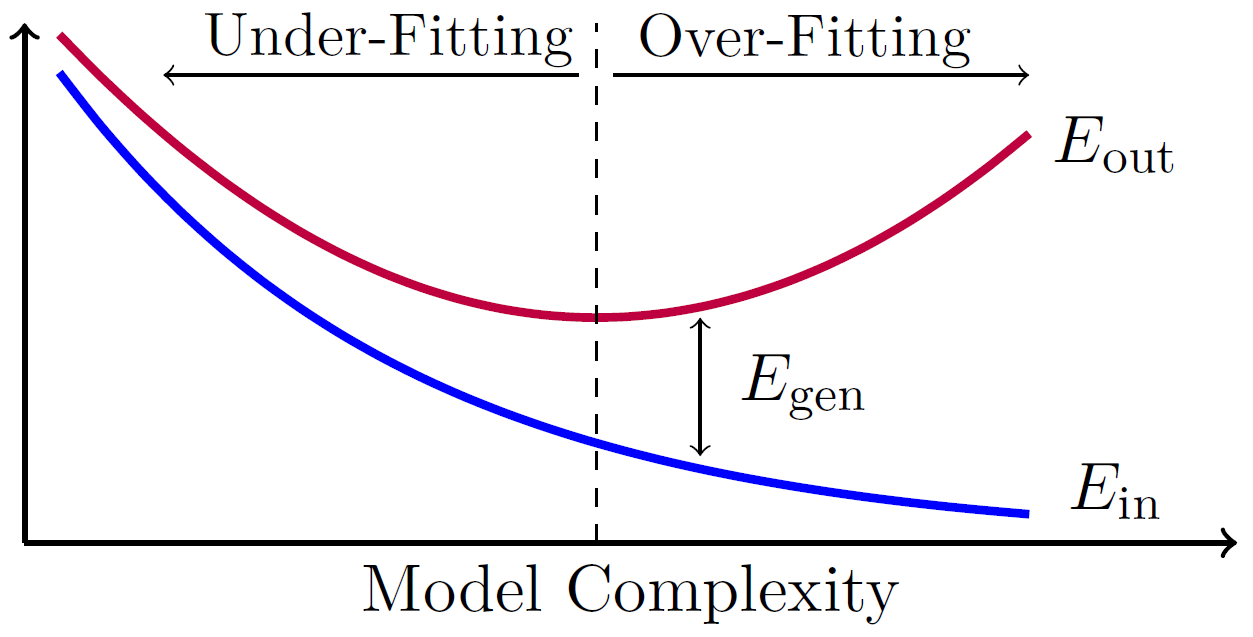
\includegraphics[width=0.6\textwidth]{images/overfitting.png}
	\caption{Overfitting and Underfitting}
	\label{fig:mesh1}
\end{figure}

\textbf{Regularization}: It refers to techniques that reduce over-fitting when learning with complex models.
\begin{equation}
	\mathcal{L}_{Reg} (\theta) = \mathcal{L} + \Omega(\theta)
\end{equation}

Popular regularziation methods can be listed as:
\begin{itemize}
	\item \textbf{Data Augmentation}
	\item \textbf{Early Stop}
	\item \textbf{Dropout}: 
	\begin{algorithm}[h]
		\SetAlgoLined
		\KwIn{mini-batch $\mathcal{B}$}
%		\KwResult{Write here the result }
%		initialization\;
		\For{$X$ $\in$ $\mathcal{B}$}{
			for earch layer, delete nodes with probability $1 - p$\;
			derive gradient with backpropagation and set the gradient of droped nodes to $0$;
		}
		average the gradients derived above and update the parameters.
		\caption{How to do dropout}
	\end{algorithm}
	\item \textbf{L1 Regularizer}: $\Omega(\theta) := \lambda_{Reg} | \theta | _2$
	\item \textbf{L2 Regularizer}: $\Omega(\theta) := \lambda_{Reg} || \theta || _2^2$
\end{itemize}

\section{Loss Functions}

\begin{itemize}
	\item \textbf{Mean Square Error}:
	\begin{equation}
		\hat{\theta} = \argmin_{\theta} ( Y - X \theta )^2
	\end{equation}
	\item \textbf{Cross Entropy}: Minimize Cross Entropy = Maximize Likelihood
	\begin{align}
		CE(\tilde{p}; p) &= - \sum_{y \in Y} \tilde{p} (y) \log p(y) \\
		&= - \mathbbm{1}_{y_i = 1} \log p_{Y|X} (1 | x_i) - \mathbbm{1}_{y_i = 0} \log p_{Y|X} (0 | x_i)
	\end{align}
	\item \textbf{Focal Loss function}
	\item \textbf{IoU Loss function}
	\item \textbf{Dice Loss function}
\end{itemize}

\section{Practical Backpropagation Method}

\subsection{Symbolic Differentiation}

This is basically the method TensorFlow uses, a.k.a computational graph.
\begin{figure}[h]
	\centering
	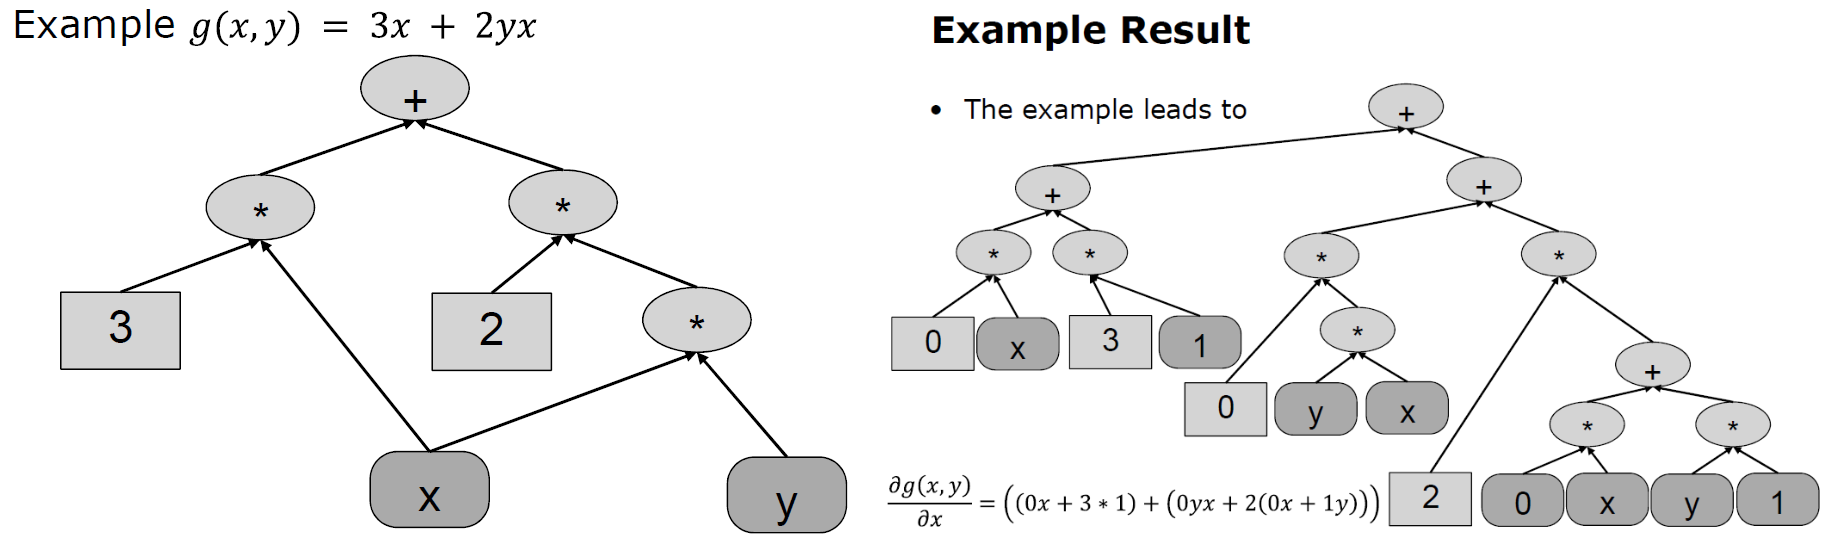
\includegraphics[width=0.9\textwidth]{images/symbolicbp.png}
	\caption{Symbolic Differentiation}
	\label{fig:symbolicbp}
\end{figure}

\subsection{Numerical Differentiation}

\begin{equation}
	\frac{\partial f(x)}{\partial x} \approx \frac{f(x + \epsilon) - f(x)}{\epsilon}
\end{equation}

\subsection{AutoDiff}

\textbf{Dual Numbers} are similar to complex numbers but replace the imaginary part with infinitesimal number $a + \epsilon b$ such that $\epsilon \neq 0$ but $\epsilon^2 = 0$.
\begin{align}
	(a + \epsilon b) + (c + \epsilon d ) = (a + c ) + \epsilon (b + d) \\
	(a + \epsilon b)(c + \epsilon d ) = ac + \epsilon (bc + ad)
\end{align}

Combined with Taylor Expansion.
\begin{align}
	f(a + \epsilon b) &= f(a) + \frac{f^{\prime} (a)}{1!} \epsilon b + \frac{f^{\prime \prime}(a)}{2!} \epsilon^2 b^2 + ... \\
	&= f(a) + \epsilon b f^{\prime} (a)
\end{align}
Reason: $\epsilon^2 = 0$. 
\begin{figure}[h]
	\centering
	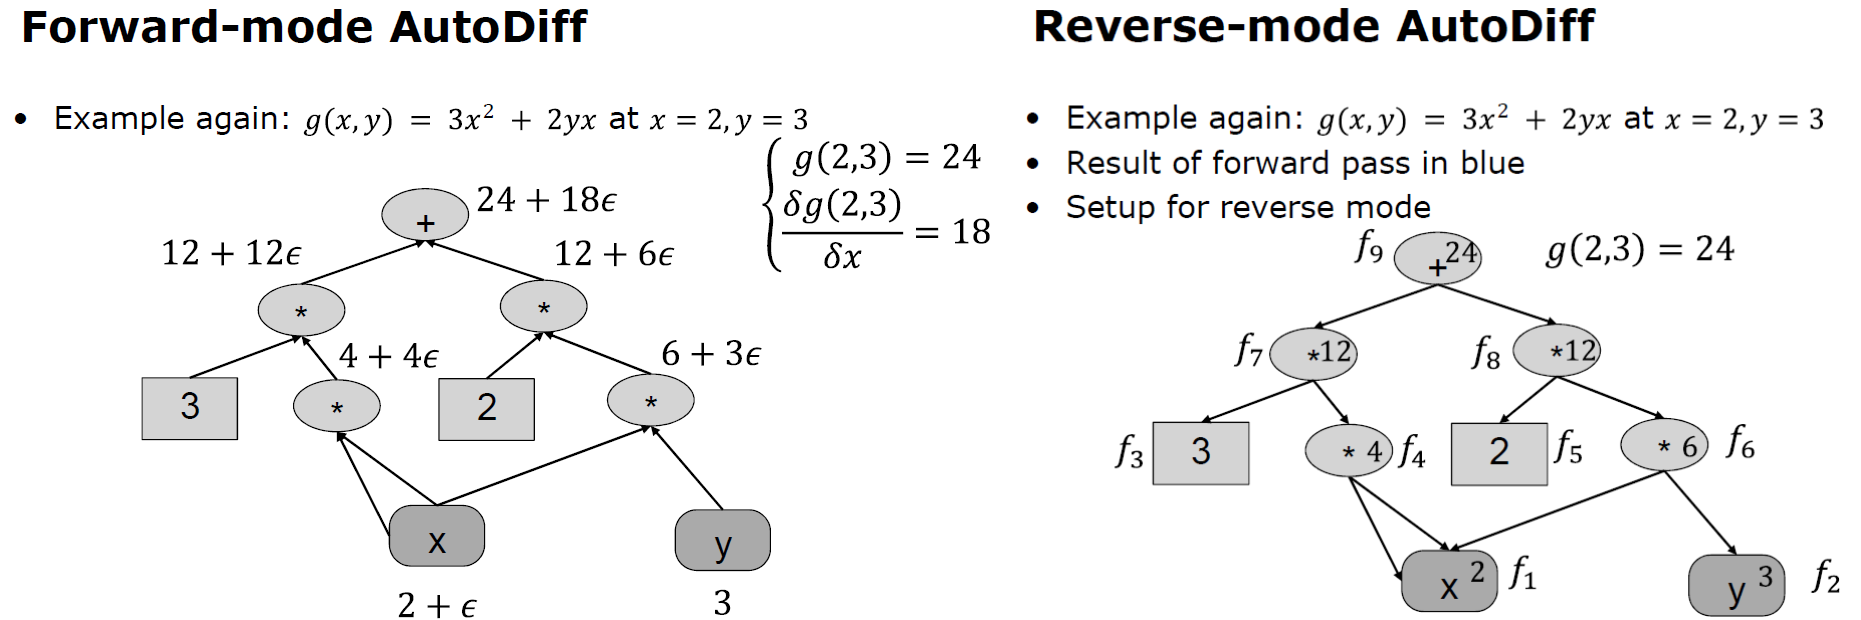
\includegraphics[width=0.9\textwidth]{images/autodiffcombine.png}
	\caption{AutoDiff}
	\label{fig:autodiff}
\end{figure}


\section{Optimization Methods}


\begin{itemize}
	\item \textbf{Gradient Descent (GD)}: Assume Dataset $\mathcal{D} = \{ x_1, x_2, ..., x_n \}$, where $n \in \mathbb{R}$.
	\begin{align}
		g_{t, t-1} &= \partial_{\theta} \sum_{i=1}^{n} f(x_i, \theta_{t-1}) \\
		\theta_{t} &\leftarrow \theta_{t-1} - \eta \cdot g_{t, t-1}
	\end{align}
	\item \textbf{Stochastic Gradient Descent (SGD)}
	\begin{align}
		g_{t, t-1} &= \partial_{\theta} f(x_i, \theta_{t-1}) \\
		\theta_{t} &\leftarrow \theta_{t-1} - \eta \cdot g_{t, t-1}
	\end{align}
	\item \textbf{Mini-batched SGD}
	\begin{align}
		g_{t, t-1} &= \partial_{\theta} \frac{1}{|\mathcal{B}|} \sum_{i \in \mathcal{B}} f(x_i, \theta_{t-1}) \\
		\theta_{t} &\leftarrow \theta_{t-1} - \eta \cdot g_{t, t-1}
	\end{align}
	\item \textbf{Momentum}
	\begin{align}
		g_{t, t-1} &= \partial_{\theta} \frac{1}{|\mathcal{B}|} \sum_{i \in \mathcal{B}} f(x_i, \theta_{t-1}) \\
		v_t &\leftarrow \beta v_{t-1} + g_{t, t-1} \\
		\theta_{t} &\leftarrow \theta_{t-1} - \eta \cdot v_{t}
	\end{align}
	\item \textbf{AdaGrad}: The $\odot$ means matrix-vector product.
	\begin{align}
		g_{t, t-1} &= \partial_{\theta} \frac{1}{|\mathcal{B}|} \sum_{i \in \mathcal{B}} f(x_i, \theta_{t-1}) \\
		s_t &\leftarrow \beta s_{t-1} + g_{t, t-1}^2	 \\
		\theta_{t} &\leftarrow \theta_{t-1} - \frac{\eta}{\sqrt{s_t + \epsilon}} \odot g_{t, t-1}
	\end{align}
	\item \textbf{Adadelta}
	\begin{align}
		g_{t, t-1} &= \partial_{\theta} \frac{1}{|\mathcal{B}|} \sum_{i \in \mathcal{B}} f(x_i, \theta_{t-1}) \\
		g_t^{\prime} &= \frac{\sqrt{\Delta x_{t-1} + \epsilon}}{\sqrt{s_t + \epsilon}} \odot g_{t, t-1} \\
		s_t &\leftarrow \gamma s_{t-1} + (1 - \gamma) g_{t, t-1}^2	 \\
		\Delta x_t &= \rho \Delta x_{t-1} + (1 - \rho) {g_t^{\prime}}^2
	\end{align}
	\item \textbf{RMSProp}
	\begin{align}
		g_{t, t-1} &= \partial_{\theta} \frac{1}{|\mathcal{B}|} \sum_{i \in \mathcal{B}} f(x_i, \theta_{t-1}) \\
		s_t &\leftarrow \gamma s_{t-1} + (1 - \gamma) g_{t, t-1}^2	 \\
		\theta_{t} &\leftarrow \theta_{t-1} - \frac{\eta}{\sqrt{s_t + \epsilon}} \odot g_{t, t-1}
	\end{align}
	\item \textbf{Adam}
	\begin{align}
		g_{t, t-1} &= \partial_{\theta} \frac{1}{|\mathcal{B}|} \sum_{i \in \mathcal{B}} f(x_i, \theta_{t-1}) \\
		v_t &\leftarrow \beta_1 v_{t-1} + (1 - \beta_1) g_{t, t-1}	 \\
		s_t &\leftarrow \beta_2 s_{t-1} + (1 - \beta_2) g_{t, t-1}^2	 \\
		\hat{v}_t &= \frac{v_t}{1 - {\beta}_1^{t}} \\
		\hat{s}_t &= \frac{s_t}{1 - {\beta}_2^{t}} \\
		\theta_{t} &\leftarrow \theta_{t-1} - \frac{\eta \hat{v}_t}{\sqrt{\hat{s}_t} + \epsilon}
	\end{align}
	\item \textbf{Newton's Method}: Hessian Matrix too big for computation.
	\begin{equation}
		\mathbb{\beta}^{t_1} \approx \mathbb{\beta}^{t_0} - \mathbb{H}^{-1} \Delta_{\beta} J (\mathbb{\beta}^{t_0})
	\end{equation}
\end{itemize}

\section{Convolutional Neural Networks (CNN)}

\subsection{Convolutional Layers}

How to calculate output size regarding input size.
\begin{equation}
	O = \frac{W - K + 2P}{S} + 1
\end{equation}
Where, $O$ is output size; $W$ input feature map size; $K$ kernel size; $P$ one-sided padding size; $S$ stride.

\subsection{``Deconvolution'' or Fractionally-Strided Convolution}

The term ``Deconvolution'' is actually fractionally-strided convolution. The stride of this type of convolution can be expressed as fractional numbers, such as $\frac{1}{2}$, $\frac{1}{3}$, and etc. An example is shown as below.
\begin{figure}[h]
	\centering
	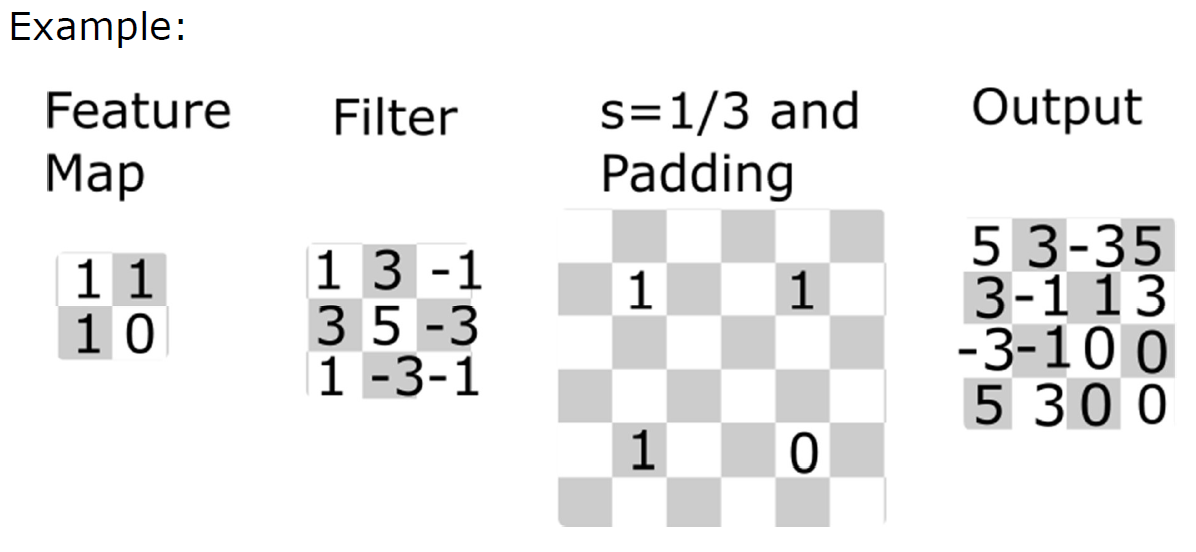
\includegraphics[width=0.6\textwidth]{images/deconv.png}
	\caption{AutoDiff}
	\label{fig:deconv2d}
\end{figure}

\subsection{Pooling Layers}

\begin{itemize}
	\item \textbf{Median Pooling}
	\item \textbf{Mean Pooling}
	\item \textbf{Max Pooling}
	\item \textbf{$L^2$ Norm Pooling}
\end{itemize}






%%%%%%%%%%%%%%%%%%%%%%%%%%%%%%%% Starting here, we shall write another one %%%%%%%%%%%%%%%%%%%%%%%%%%%%%%%

%\subsection{Backbones}
%
%\begin{itemize}
%	\item \textbf{Xception}
%	\item \textbf{VGG16}
%	\item \textbf{ResNet50}
%	\item \textbf{InceptionV3}
%	\item \textbf{MobileNet}
%	\item \textbf{DenseNet}
%	\item \textbf{NASNet}
%\end{itemize}
%
%\subsection{Neck Layers}
%
%\begin{itemize}
%	\item \textbf{Feature Pyramid Networks (FPN)}
%\end{itemize}
%
%\subsection{Data Augmentation}
%
%\begin{itemize}
%	\item \textbf{Point Operations}: Change brightness, saturation, hue, gamma, correction, histogram equalization, etc.
%	\item \textbf{Geometric Operations}: Shift, flip, rotate or shear.
%	\item \textbf{Adding Noise}: Gaussian noise, etc.
%\end{itemize}
%
%\section{Object Detection}
%
%\subsection{One-Stage Detector}
%
%\begin{itemize}
%	\item \textbf{YOLO}
%	\item \textbf{SSD}
%\end{itemize}
%
%\subsection{Two-Stage Detector}
%
%\begin{itemize}
%	\item \textbf{Faster R-CNN}: \textbf{Region Proposal Networks} + \textbf{Classification Head}; It is an anchor-based method.
%\end{itemize}
%
%\subsection{Metrics}
%
%\begin{itemize}
%	\item \textbf{Precision}:
%	\begin{equation}
%		\text{precision} = \frac{TP}{TP +_ FP}
%	\end{equation}
%	\item \textbf{Recall}:
%	\begin{equation}
%		\text{recall} = \frac{TP}{TP + FN}
%	\end{equation}
%	\item \textbf{Average Precision (AP)}: the area of precision-recall curves.
%	\item \textbf{F1 Score}:
%	\begin{equation}
%		F1 = \frac{2}{\frac{1}{\text{precision}} + \frac{1}{\text{recall}}} = \frac{TP}{TP + \frac{FN + FP}{2}}
%	\end{equation}
%	\item \textbf{Receiver Operating Characteristics (ROC) Curves}:
%	\begin{align}
%		TPR &= \frac{TP}{TP + FN} \\
%		FPR &= \frac{FP}{TN + FP}
%	\end{align}
%	\item \textbf{Confusion Matrix}: assume a classification task, the confusion matrix is computed on the validation set with each entry of the matrix indicating the count for each class predicted by the classifier. Example shown as below.
%	\begin{equation}
%		C = 
%		\begin{bmatrix}
%			21 & 2 & 7 \\
%			10 & 11 & 9 \\
%			3 & 1 & 26 \\
%		\end{bmatrix}
%	\end{equation}
%	Where, the perfect classifier would have results like,
%	\begin{equation}
%		C = 
%		\begin{bmatrix}
%			30 & 0 & 0 \\
%			0 & 30 & 0 \\
%			0 & 0 & 30 \\
%		\end{bmatrix}
%	\end{equation}
%\end{itemize}
%
%\section{Image Segmentation}
%
%\subsection{Instance Segmentation}
%
%\begin{itemize}
%	\item \textbf{Mask R-CNN}
%	\item \textbf{YOLACT}
%	\item \textbf{SOLO}
%\end{itemize}
%
%\subsection{Semantic Segmentation}
%
%\begin{itemize}
%	\item \textbf{SegNet}
%	\item \textbf{FCN}
%	\item \textbf{U-Net}
%\end{itemize}
%
%\subsection{Metrics}

%%%%%%%%%%%%%%%%%%%%%%%%%%%%%%%%%%%%%%%%%%%%%%%%%%%%%%%%%%%%%%%%%%%%%%%%%%%%%%%%%%%%%%%%%%%%%%%%%


%\bibliographystyle{acm}
%\bibliography{bibliography}
\end{document}